\chapter{Sampling} \label{ch:sampling}

The data used for statistics analysis is usually a small portion collected from a huge group. The collected data is called a sample, and the huge group from which the sample is collected, the population. For example, the incomes of a random 1000 citizens as a sample may reflect the incomes of the entire city. Another example is that the working efficiency of a machine for the past months as a sample may reflect its working efficiency in its entire lifespan.

An important underlying assumption behind statistics is that the insights observed from the sample also apply to the population. With that regard, questions naturally come up. Why does this assumption hold? When does this assumption hold? In what extend does this assumption hold? What can be done to make the sample more effective and efficient when reflecting the population?

This chapter tries to answer the above questions. As it is introduced later, the inference from sample to population is not certain, as there is a chance (however small it might be) that the samples are completely biased from the population. Therefore, we must use probability in any statement drawn from statistics analysis.

\section{Sampling Methods}

When selecting elements from the population, make sure that all elements have a equal probability of being selected, hence, random sampling. Depending on how many times a member can be sampled, we have
\begin{itemize}
  \item Sampling with replacement: a member can be chosen more than once.
  \item Sampling without replacement: a member can be chosen no more than once.
\end{itemize}

Sometimes it is interesting to compare the differences of the two methods, especially then the population is finite. An obvious difference is that by using sampling with replacement all the samples can be considered as ``independent event'', while by using sampling without replacement, previous samples may change the distributions in the remaining population, thus making the samples relevant. In this case, using sampling with replacement can theoretically be considered as sampling from an infinite population (by thinking that the population is duplicated as many times as necessary).

In practice, the population is usually so large, that sampling from a finite population can be considered as sampling from an infinite population, and the two methods would make no differences as far as it is concerned.

Consider the following examples. A set of $N$ random variables are generated from a Gaussian distribution as the population. Sample the population $M$ times using sampling with replacement and sampling without replacement, respectively. Calculate the sampled mean and variance after each sampling instance, and see how it converges to the mean and variance of the population.

In the first example, let $N=100$ and $M=500$. Figures \ref{ch:sampling:fig:sample-wr-n100} and \ref{ch:sampling:fig:sample-nwr-n100} gives the cumulative mean and variance of sampling with and without replacement, respectively. The mean and variance are given by red and blue curves, respectively. The statistics obtained from the cumulative samples and from the population are given by the solid and dashed curves, respectively. Notice that in Fig. \ref{ch:sampling:fig:sample-nwr-n100}, after number of samples exceeding $100$, the entire population has been sampled, and thus the sampling stops. This explains why its mean and variance stop fluctuating and converge to the population mean and variance, respectively.

\begin{figure}
	\centering
	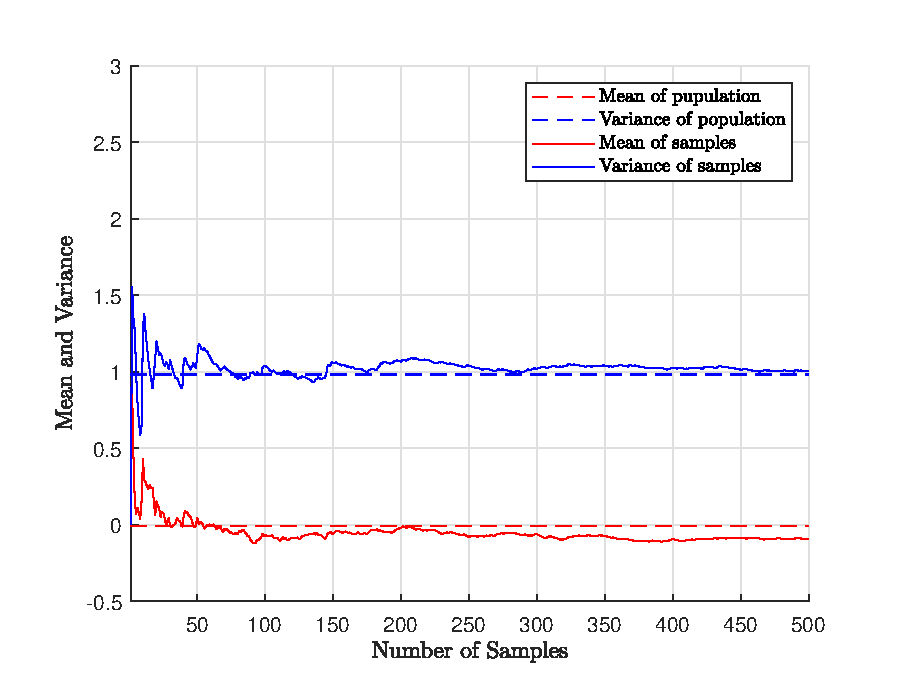
\includegraphics[width=250pt]{chapters/ch-sampling/figures/sample-wr-n100.eps}
	\caption{Sample with replacement, $N=100$, $M=500$.} \label{ch:sampling:fig:sample-wr-n100}
\end{figure}

\begin{figure}
	\centering
	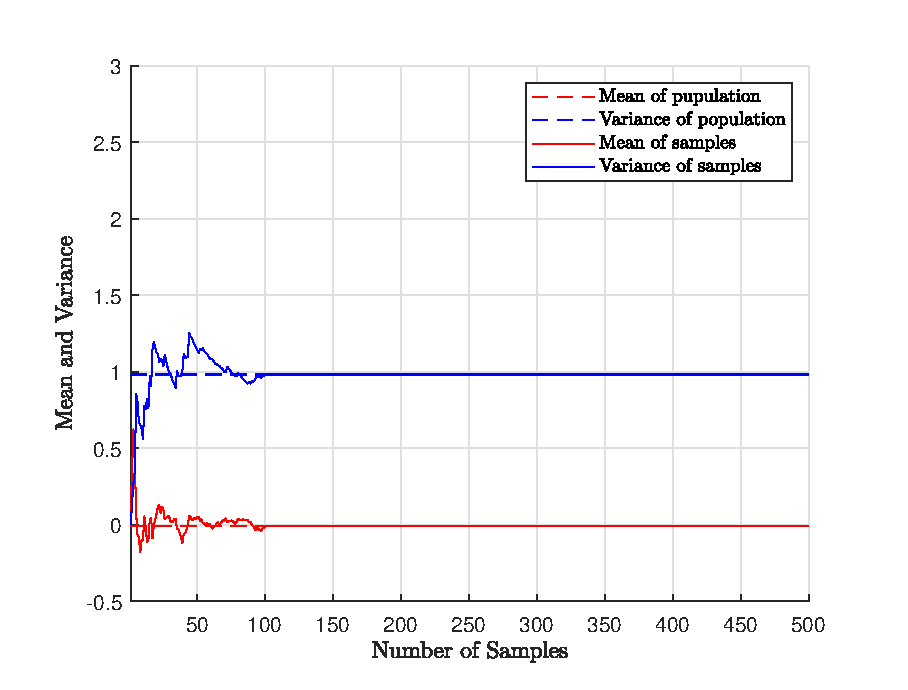
\includegraphics[width=250pt]{chapters/ch-sampling/figures/sample-nwr-n100.eps}
	\caption{Sample without replacement, $N=100$, $M=500$.} \label{ch:sampling:fig:sample-nwr-n100}
\end{figure}

In practice, however, the population size is often orders of magnitudes larger than the number of samples. In the second example, let $N=10000$ and $M=500$. The corresponding figures are given in Figs. \ref{ch:sampling:fig:sample-wr-n10000} and \ref{ch:sampling:fig:sample-nwr-n10000}. There is no obvious differences of the two figures from statistics perspective.

\begin{figure}
	\centering
	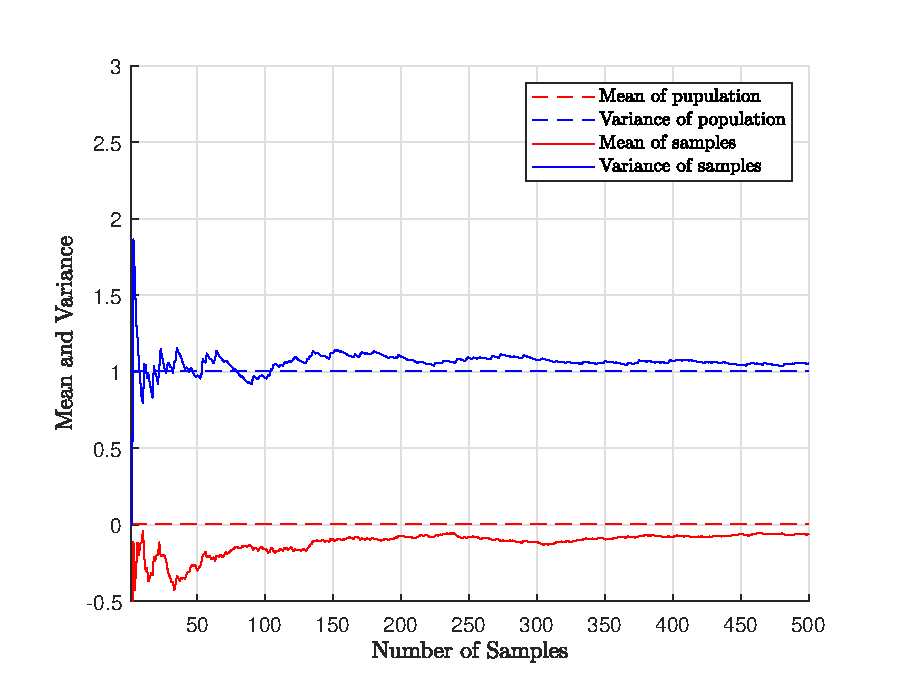
\includegraphics[width=250pt]{chapters/ch-sampling/figures/sample-wr-n10000.eps}
	\caption{Sample with replacement, $N=10000$, $M=500$.} \label{ch:sampling:fig:sample-wr-n10000}
\end{figure}

\begin{figure}
	\centering
	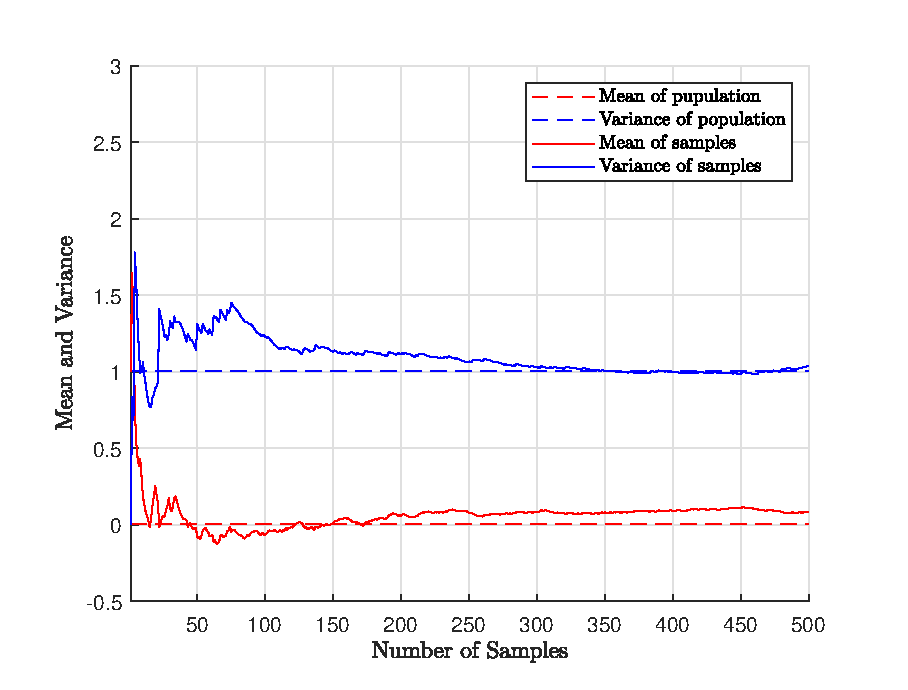
\includegraphics[width=250pt]{chapters/ch-sampling/figures/sample-nwr-n10000.eps}
	\caption{Sample without replacement, $N=10000$, $M=500$.} \label{ch:sampling:fig:sample-nwr-n10000}
\end{figure}

\section{Model of Population}

The features of the population is often not known, or at least not known entirely. It is possible to make some preliminary assumptions to the distribution of population, with parameters to be further confirmed using the samples.

For example, let $X$ be a variable of the population. It could be, for example, the heights of all teenagers in a city. We can make an assumption that $X$ follows some distribution $f(x)$. A widely used assumption, in this scenario, is that $f(x)$ is a Gaussian distribution with mean $\mu$ and standard deviation $\sigma$, and each element in the population, $X_i$, can be taken as a random variable generated from $f(x)$. In the case of Gaussian distribution, since it is uniquely characterized by $\mu$ and $\sigma$, other quantities such as the median, moments, skewness, etc., can be derived once $\mu$ and $\sigma$ is calibrated.

The questions rise sequentially are:
\begin{itemize}
  \item What are the parameters in the assumed distribution?
  \item Does it indeed follow the assumed distribution?
\end{itemize}
The answers to the above questions need to be found out via the samples, or more precisely, from the sample statistics.

\section{Sample Statistics}





